\documentclass[a4paper,12pt]{article}
    \usepackage{listing}
    \usepackage{graphicx}
    \begin{document}
    
    
\title{7. Implementation of client server communication using socket programming and UDP as transport layer protocol}
\author{Santhisenan A}
\date{\today}
\maketitle
    
\section{Socket Programming}
    
\subsection{Socket}
A socket is one of the most fundamental technologies of computer network programming. Sockets allow network software applications to communicate using standard mechanisms built into network hardware and operating systems.
    
    
A socket represents a single connection between exactly two pieces of software (a so-called point-to-point connection). More than two pieces of software can communicate with client/server or distributed systems by using multiple sockets. For example, many Web browsers can simultaneously communicate with a single Web server via a group of sockets made on the server.
    
    
Socket-based software usually runs on two separate computers on the network, but sockets can also be used to communicate locally (interprocess) on a single computer. Sockets are bidirectional, meaning that either side of the connection is capable of both sending and receiving data. Sometimes the one application that initiates communication is termed the "client" and the other application the "server," but this terminology leads to confusion in peer to peer networking and should generally be avoided.
    
\subsection{Socket Interface Types}
    
Socket interfaces can be divided into three categories:
    
\begin{itemize}
	\item \textit{Stream sockets}, the most common type, requires that the two communicating parties first establish a socket connection, after which any data passed through that connection will be guaranteed to arrive in the same order in which it was sent - so-called connection-oriented programming model.
	\item \textit{Datagram sockets} offer "connection-less" semantics. With datagrams, connections are implicit rather than explicit as with streams. Either party simply sends datagrams as needed and waits for the other to respond; messages can be lost in transmission or received out of order, but it is the application's responsibility and not the sockets to deal with these problems. Implementing datagram sockets can give some applications a performance boost and additional flexibility compared to using stream sockets, justifying their use in some situations.
	\item The third type of socket -- \textit{the raw socket} -- bypasses the library's built-in support for standard protocols like TCP and UDP. Raw sockets are used for custom low-level protocol development.
\end{itemize}
    
\subsection{Socket support in network protocols}
Modern network sockets are typically used in conjunction with the Internet protocols -- IP, TCP, and UDP. Libraries implementing sockets for Internet Protocol use TCP for streams, UDP for datagrams, and IP itself for raw sockets.
    
    
To communicate over the Internet, IP socket libraries use the IP address to identify specific computers. Many parts of the Internet work with naming services, so that the users and socket programmers can work with computers by name (e.g., "thiscomputer.wireless.about.com") instead of by address (e.g., 208.185.127.40).
    
    
Stream and datagram sockets also use IP port numbers to distinguish multiple applications from each other. For example, Web browsers on the Internet know to use port 80 as the default for socket communications with Web servers.
    
    
\section{UDP}
In computer networking, the User Datagram Protocol (UDP) is one of the core members of the Internet protocol suite. The protocol was designed by David P. Reed in 1980 and formally defined in RFC 768. With UDP, computer applications can send messages, in this case referred to as datagrams, to other hosts on an Internet Protocol (IP) network. Prior communications are not required in order to set up communication channels or data paths.

UDP uses a simple connectionless communication model with a minimum of protocol mechanism. UDP provides checksums for data integrity, and port numbers for addressing different functions at the source and destination of the datagram. It has no handshaking dialogues, and thus exposes the user's program to any unreliability of the underlying network; There is no guarantee of delivery, ordering, or duplicate protection. If error-correction facilities are needed at the network interface level, an application may use the Transmission Control Protocol (TCP) or Stream Control Transmission Protocol (SCTP) which are designed for this purpose.
    
UDP is suitable for purposes where error checking and correction are either not necessary or are performed in the application; UDP avoids the overhead of such processing in the protocol stack. Time-sensitive applications often use UDP because dropping packets is preferable to waiting for packets delayed due to retransmission, which may not be an option in a real-time system.    
\section{Code} 
\subsection{client.py}
\begin{verbatim}
        import socket

        UDP_IP = "127.0.0.1"
        UDP_PORT = 5005
        MESSAGE = "Hello, World!"
        
        print "UDP target IP:", UDP_IP
        print "UDP target port:", UDP_PORT
        print "message:", MESSAGE
        
        sock = socket.socket(socket.AF_INET, # Internet
                             socket.SOCK_DGRAM) # UDP
        sock.sendto(MESSAGE, (UDP_IP, UDP_PORT))
\end{verbatim}
\subsection{server.py}
\begin{verbatim}
        import socket

        UDP_IP = "127.0.0.1"
        UDP_PORT = 5005
        
        sock = socket.socket(socket.AF_INET, # Internet
                             socket.SOCK_DGRAM) # UDP
        sock.bind((UDP_IP, UDP_PORT))
        
        while True:
            data, addr = sock.recvfrom(1024) # buffer size is 1024 bytes
            print "received message:", data
\end{verbatim}
    
\section{Output}

\pagebreak
\begin{figure}
	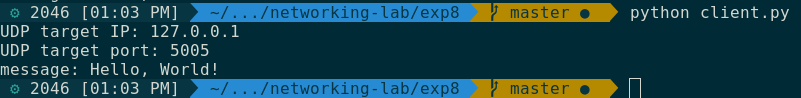
\includegraphics[width=\linewidth]{./client-udp.png}
	\caption{Client}
	\label{fig:client}
\end{figure}

\begin{figure}
	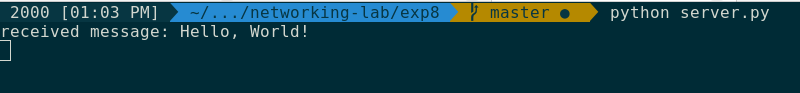
\includegraphics[width=\linewidth]{server-udp.png}
	\caption{Server}
	\label{fig:server}
\end{figure}
    
\end{document}